\label{sec:materials_and_methods}
% \clearpage
test
\subsection{State of the Art}\label{subsec:state-of-the-art}
The transient electromagnetic (TEM) method is a time-domain electromagnetic technique
widely used for exploring the subsurface, providing valuable insights into environmental
applications like groundwater detection.
Interpreting TEM data effectively requires solid inversion techniques,
and the L-curve method stands out for helping balance the fit of the data with the complexity of the model.

\subsubsection{Common resistivity values}\label{subsubsec:common-resistivity-values}
Electrical resistivity is a key parameter in geophysical investigations, as it provides valuable information about the properties of the Earth's subsurface.
Many electrical and electromagnetic methods rely on constructing a model of the electrical resistivity distribution to characterise subsurface materials.
By analysing these resistivity values, it is possible to infer the composition of subsurface layers
and detect geological structures such as faults, fractures, and aquifers~\parencite{christiansen2006transient}.

\begin{table}[h]
    \centering
    \caption{Common Resistivity Values of Subsurface Materials}

\resizebox{\columnwidth}{!}{
    \begin{tabular}{l c}
        \hline
        \textbf{Material} & \textbf{Resistivity ($\Omega\text{m}$)} \\
        \hline
        Saturated layers with high salinity & 0.1 – 5 \\
        Saturated clays and silts & 5 – 15 \\
        Saturated sediments & 10 – 20 \\
        Unsaturated sediments & 50 – 80 \\
        Saturated sand & 40 – 150 \\
        Unsaturated sand & 400 – 1500 \\
        \hline
    \end{tabular}
    }
    \label{tab:resistivity}
\end{table}

\cref{tab:resistivity} presents commonly reported resistivity values for different subsurface materials.
These values have been compiled from multiple studies conducted in diverse geological settings and
using various geophysical methods~\parencite{gomez2019alluvial, galazoulas2015large, george2021modelling}.

In the context of~\cref{tab:resistivity}, the term ``sediments'' refers to unconsolidated deposits consisting of a mixture of sand, silt, and clay.
The precise resistivity values presented in~\cref{tab:resistivity} for sediments are not general global values but are
specific to the study region investigated by \textcite{gomez2019alluvial}.
These values reflect the characteristics of sediments found in the Challapampa aquifer in Bolivia,
where variations in grain size, moisture content, and mineral composition influence the resistivity measurements.

\subsubsection{Transient Electromagnetic method}\label{subsubsec:tem-method}
The transient electromagnetic (TEM) method is a geophysical technique developed for subsurface exploration and mineral prospecting in the 1980s.
It is a time-domain electromagnetic method that can be used to infer information about the electrical conductivity distribution of the Earth's subsurface.
As an electromagnetic wave propagates through the subsurface, it is attenuated by the electrical properties of the materials it encounters.
The Maxwell equations govern that a changing electrical field induces a magnetic field, and vice versa.
For the TEM method a pulse of current is transmitted through a transmitter loop generating a primary magnetic field.
When the current is turned off, the decay of the primary field induces secondary currents (eddy currents) in the ground,
which produce a secondary electromagnetic field.
This field is measured using a receiver coil, as the strength of the secondary field depends on the conductivity of the material the EM wave propagates through.
By analysing the decay characteristics of the secondary field, it is possible to infer the conductivity structure of the subsurface,
because the wave propagates deeper into the subsurface, later times include information about deeper layers.
Such a decay curve is called a transient and multiple transients are measured for each sounding to counteract the random noise in the measurement.
An EM wave attenuates faster in conductive materials, which results in a shallower investigation depth.
For this reason the TEM method was developed to find conductive materials like ores, clay, and water-bearing formations in resistive media.
As the interpretation of the data is computationally intensive and requires sophisticated instruments to measure the secondary field accurately,
this method is rather ``young'' compared to other geophysical methods like electrical resistivity tomography (ERT) and magnetotellurics (MT)~\parencite{christiansen2006transient}.

In order to get information on the subsurface resistivity, the measured signal must be converted to an apparent resistivity ($\rho_a$).
This can be done by using the formula for late stage behaviour of the secondary field:
\begin{equation}
    \rho_a = \frac{1}{\pi} \left( \frac{M}{20 \cdot \frac{\partial b_z}{\partial t}} \right)^{\frac{2}{3}} \left( \frac{\mu_0}{t} \right)^{\frac{5}{3}}
    \label{eq:apparent_resistivity}
\end{equation}
where $M$ is the magnetic moment, $\frac{\partial b_z}{\partial t}$ is the signal measured by the receiver coil,
$\mu_0$ is the magnetic permeability of free space and $t$ is the time.
The magnetic moment is the product of the number of turns, the area, and the current in the transmitter loop.
The apparent resistivity is a measure of the resistivity of the subsurface material the EM wave has traveled through,
but it is not the true resistivity of the material.
For this reason inflection points can be interpreted as boundaries between different layers with different resistivities,
and the slope of the curve shows whether the resistivity is increasing or decreasing in the new layer~\parencite{fitterman1986transient}.

\begin{figure*}[ht]
    \centering
    \includegraphics[width=\textwidth]{data/20240522/TEM-data/08-forward_model/example_response}
    \caption{Numerically modelled typical TEM response with the signal a) and the apparent resistivity b).}
    \label{fig:typical_sounding}
\end{figure*}

Another approach is to use the inversion of the data to create a model of the subsurface resistivity.
This is explained in more detail in~\cref{subsubsec:data-inversion}.
For the interpretation of TEM data -- and for the inversion in particular -- some assumptions must be made:
EM waves only propagate vertically and the subsurface is layered.
As most inversion algorithms are work with a 1D model, the subsurface is assumed to be homogeneous in the horizontal direction.
Even with these limitations the TEM method is a powerful tool for the
exploration of the subsurface and can be used in various applications~\parencite{christiansen2006transient}.

\subsubsection{Environmental applications of TEM}\label{subsubsec:application-of-tem}
Although the TEM method originates from the mining industry, it can have various environmental applications,
the most common being exploration and characterisation of groundwater resources is one of the most common applications of the TEM method.

In this context, \textcite{danielsen2003application} used the TEM method for the exploration of buried valleys as potential aquifers in Denmark.
The study introduced two new TEM systems based on the Geonics PROTEM -- the high moment transient electromagnetic (HiTEM) system for a deeper investigation depth
and the pulled array Transient electromagnetic (PATEM) system for a higher lateral resolution.
The HiTEM system uses a combination of a $30\times30\,\text{m}$ transmitter loop and a current of $75\,\text{m}$ to achieve a depth of investigation (DOI) of up to $300\,\text{m}$.
To mitigate distortion effects, an offset receiver loop is used for the later times and a central receiver loop with a reduced current of $2.5\,\text{A}$ for the early times.
A mutually constrained inversion (MCI) is used to invert the combination of the data gathered with the two different configurations.
The PATEM system uses a $3\times5\,\text{m}$ transmitter loop on a wheeled frame with an offset receiver loop.
This allows for continuous measurements along a profile and a DOI of $100-150\,\text{m}$.
To achieve a high DOI and useful near surface information, the PATEM system allows for a transmitter configuration with either 2 turns with $16\,\text{A}$ or 8 turns with $40-50\,\text{A}$.
The study also touches on the problems resulting from coupling with man-made structures.
The coupling effects can be divided into galvanic and capacitive.
Galvanic coupling is caused by grounded conductors like power lines and causes an underestimation of the resistivity.
Capacitive coupling is caused by current being generated in the conductor and leaking into the ground through an insulation, which leads to an oscillating signal.
For this reason the study recommends keeping a distance of about $150\,\text{m}$ from underground cables or pipes when the earth has a resistivity of $40-50\,\Omega\text{m}$.
The study finds that a 1D inversion approach is sufficient to detect the slope of a 2D buried valley when in a layer with low resistivity.
In a layer with high resistivity, only the overall structure of the valley can be derived.

Similarly to the PATEM system, \textcite{auken2019ttem} propose a towed transient electromagnetic (tTEM) system for an efficient 3D mapping of the subsurface.
The tTEM system utilises a $2\times4\,\text{m}$ transmitter loop mounted on a non-conductive sled towed by an vehicle, which enables a production rate of about $1\,\text{km}^2$ per day.
The receiver loop is towed at $9\,\text{m}$ offset from the transmitter.
Like the PATEM system, the tTEM system permits the use of two different currents ($2.8~\text{and}~30\,\text{A}$) in order to gain a relatively high DOI of up to $70\,\text{m}$,
while still allowing the investigation of shallow depths.
This study also highlights the importance of considering the coupling effects of the system with conductive objects
and it tests the system in an environment with a high resistivity of the subsurface ($>600\,\Omega\text{m}$).
Under these circumstances the signal caused by coupling can be observed in isolation
and the study found that a minimal distance of $3\,\text{m}$ between transmitter and vehicle was necessary to mitigate coupling effects.
As it is important to calibrate TEM systems, the tTEM system was validated at the Danish National TEM test site.
Furthermore, the tTEM system was also validated against borehole data and the results showed a good agreement.

Electromagnetic methods do not require direct contact with the subsurface, which allowed for the development of airborne electromagnetic methods (AEM).
\textcite{sorensen2004skytem} introduced the SkyTEM system as an alternative to ground based TEM systems.
The SkyTEM system uses a helicopter to carry a $12.5\times12.5\,\text{m}$ transmitter loop with 4 turns and a receiver loop ($0.5\times0.5\,\text{m}$) in a central configuration.
Just like the PATEM and HiTEM systems, a low moment and a high moment configuration are used to achieve a high DOI while still resolving the near surface layers.
In the low moment configuration the current of $35\,\text{A}$ only flows through one turn and for the high moment $50\,\text{A}$ are used with all 4 turns.
The SkyTEM system was validated against a ground based TEM system with a transmitter loop size of $40\times40\,\text{m}$, showing a good agreement (below 5\% deviation).
This system is able to cover a larger area than traditional ground based systems in the same amount of time, while still being able to resolve underground structures,
such as buried valleys.

To investigate the subsurface below continental bodies of water, \textcite{aigner2021flexible} propose a flexible single loop system which can be towed by a boat.
By using a single loop which is kept afloat by several PVC pipe segments that keep it in a circular shape, the system can easily be moved around the lake.
Using pipe segments allows for different loop sizes and thus different investigation depths.
The TEM-FAST~48 system by Applied Electromagnetic Research (AEMR) was used to investigate the subsurface of the Lake Langau in Austria.
A current of $4\,\text{A}$ and loops with radii between $6.2-11.9\,\text{m}$ were used, leading to an investigation depth between $6.2-50.0\,\text{m}$,
which was sufficient to detect sedimentary layers below the lake.
For a proper interpretation of early time data, it is important to understand how long the turn-off time of the transmitter for a single-loop setup is.
When the transmitter is turned off, the current in the loop takes a certain amount of time to decay, which is called the turn-off ramp.
This time was measured to be between $4.2-10.4\,\mu\text{s}$ -- depending on loop size and resistivity of the subsurface.
Using this information, a formula was derived to find the minimum effective sounding depth:
\begin{equation}
    h_{\text{eff}} = \sqrt{t_{\text{eff}}\overline{\rho}}
    \label{eq:h_eff}
\end{equation}
where $h_{\text{eff}}$ is the minimum effective sounding depth, $t_{\text{eff}}$ is the minimum effective time
and $\overline{\rho}$ is the average resistivity of the smooth subsurface model.
The study also showcased two different approaches to finding the DOI\@.
The first uses different starting models for the inversion assuming that the DOI is reached
when the data does not influence the inverted model anymore and will keep the values of the starting model.
The second approach is based on:
\begin{equation}
    \text{DOI} \approx 0.55(\frac{M\times\overline{\rho}}{\eta})
    \label{eq:doi}
\end{equation}
where $M$ is the magnetic moment, $\overline{\rho}$ is the average resistivity of the smooth subsurface model and $\eta$ is the noise level.
Both methods agree on a DOI ranging between 20 and 50~m depending on the loop size.

As other water sources become less reliable in some regions in Bolivia, \textcite{gonzales2018delimiting}
show the potential of the TEM method for the exploration of groundwater in the Punata alluvial fan.
This aquifer is an important water source, but it has zones with high salinity, which poses challenges in its use.
This study used the ABEM~WalkTEM system with a $50\times50\,\text{m}$ transmitter loop with a current of $18\,\text{A}$ and
two receiver loops ($0.5\times0.5\,\text{m}$ and $10\times10\,\text{m}$) in a central configuration.
This way a DOI of up to $200\,\text{m}$ was achieved in some regions of the alluvial fan, while in other regions the DOI was limited to $80\,\text{m}$.
The study was able to detect zones with high salinity and the results were validated with borehole data.

\textcite{gomez2019alluvial} conducted a similar study in the Challapampa area, Bolivia.
In this study the same WalkTEM system and loop sizes were used as in the study by Gonzales et al.\cite{gonzales2018delimiting}
However, the receiver loops were deployed in an offset configuration and
for the $0.5\times0.5\,\text{m}$ loop only a current of $2\,\text{A}$ was used, while the whole $18\,\text{A}$ were applied for the $10\times10\,\text{m}$ loop.
This setup achieved a depth of investigation (DOI) of up to $250\,\text{m}$
and identified the influence of a hot spring, which appeared as a low-resistivity zone, indicating higher salinity.

Another application of TEM is the detection of karstic features, like caves, faults, and fracture zones~\parencite{zhou2022multi, su2024response}.
Traditionally, a large transmitter loop size in the order of $100\,\text{m}$ side length was used to achieve a high investigation depth.
For this reason the TEM method was not suitable for the application in mountainous regions.
However, a similar investigation depth can be achieved by using a smaller transmitter loop size and more turns.
A multi-turn setup has the disadvantage of mutual inductance caused by the large number of turns, which can lead to underestimation of the resistivity of the subsurface.

\textcite{zhou2022multi} proposed a coincident configuration with a $2\times2\,\text{m}$ and 10 turns for the transmitter loop and 20 turns for the receiver loop.
In order to mitigate the effects of the mutual inductance, borehole and electrical resistivity tomography (ERT) data were used to constrain the inversion.
Because boreholes and ERT measurements are expensive and time-consuming,
they are only used to correct the TEM soundings in order to account for shifted resistivity values.
This method was used to detect a karst channel in Zhijin, China.

A more in-depth study on how to deal with self and mutual inductance was conducted by \textcite{su2024response}.
Here a central loop configuration (receiver loop in the centre of the transmitter loop) was compared with a multi-turn small fixed-loop configuration
(using multiple different receiver positions, while keeping the transmitter loop fixed).
For the fixed-loop set up a correction coefficient was introduced to account for off-centre receiver positions.
5 model tests were conducted in order to compare the two configurations and the results showed that after correction the fixed-loop configuration
was more accurate in detecting the position of one or multiple anomalies.

\subsubsection{Data Inversion}\label{subsubsec:data-inversion}
A typical geophysical problem can be defined as follows:
\begin{equation}
    \mathbf{d} = \mathcal{F}(\mathbf{m})
    \label{eq:geophysical_problem}
\end{equation}
where $\mathbf{d}$ is the observed data, $\mathcal{F}$ is the forward operator, and $\mathbf{m}$ is the model.
If the model is known, the forward operator can be used to calculate the expected data.
Unfortunately, usually the model is unknown and the observed data is used to find the model, which is called an inverse problem.
In practise the observed data is contaminated with noise, which introduces an error term into the equation
and makes the inversion ill-posed and non-linear.
An ill-posed problem means that small changes in the observed data can cause large differences in the model.
As a result, noise introduces variability, making it impossible to find a unique solution~\parencite{zhdanov2002geophysical}.

Approaches to address this issue can be divided into deterministic and stochastic methods.
The deterministic approach tries to find a single solution, by iteratively updating the model parameters
to minimise the difference between observed and modeled data.
To prevent overfitting to noise, Tikhonov regularisation is used, which adds a penalty term to the least squares problem.
\begin{equation}
    \| \mathbf{W}_d (\mathcal{F}(\mathbf{m}) - \mathbf{d}) \|_2^2 + \lambda \| \mathbf{W}_m (\mathbf{m} - \mathbf{m}_0) \|_2^2 \to \min
    \label{eq:tikhonov}
\end{equation}
$\mathbf{W}_d$ and $\mathbf{W}_m$ are weighting matrices, $\mathbf{m}_0$ is the initial model, and $\lambda$ is the regularisation parameter.
$\| \mathbf{W}_m (\mathbf{m} - \mathbf{m}_0) \|_2^2$ can be interpreted as the roughness of the model, which quantifies the complexity or variation of the model.
$\| \mathbf{W}_d (\mathcal{F}(\mathbf{m}) - \mathbf{d}) \|_2^2$ is the data misfit, which quantifies the difference between observed and modeled data and can include an error term.
With the choice of $\lambda$, the trade-off between data misfit and model complexity can be controlled.
Building on this foundation, several deterministic methods have been developed, such as Gauss-Newton inversion and Conjugate Gradient.
A constraint inversion can be used to incorporate prior information about the model, which can be useful to prevent overfitting to noise.
Stochastic methods, on the other hand, randomly search the solution space and provide a range of plausible models rather than a single deterministic solution.
This is significantly more computationally expensive, but can be more robust against noise and can provide uncertainty estimates.
Particle swarm optimization (PSO) and Bayesian inversion are examples of stochastic methods~\parencite{rucker2017pygimli, xue2020development}.

An implementation of the deterministic approach is the PyGIMLi library, introduced by \textcite{rucker2017pygimli},
which uses Gauss-Newton inversion to iteratively update the model parameters.
PyGIMLi is an open-source library written in Python and C++ and is designed for the inversion of geophysical data.
It allows the implementation of any given forward operator into the inversion algorithm,
which makes it a versatile tool for geophysical modeling and inversion.

\subsubsection{L-curve method}\label{subsubsec:l-curve-method}
Solving inverse problems is a task not limited to geophysics, which makes inversion theory an important field in mathematics.
There are several methods to solve an inverse problem, but the most common approach is to use Tikhonov regularisation~\eqref{eq:tikhonov}.
But the choice of the regularisation parameter $\lambda$ is not trivial and can have a significant impact on the inversion result.

The L-curve method is widely used to determine the optimal $\lambda$ for the solution of an inverse problem~\parencite{hansen1999curve}.
The L-curve is a graph of the residual norm against the solution norm.
With an increasing $\lambda$, the residual norm is expected to increase and the solution norm is expected to decrease.
This leads to a curve that resembles an L-shape.
An optimal $\lambda$ should minimise the residual norm while keeping the solution norm small.
This leads to the ``corner'' of the L, which is also the point with the highest curvature.

\textcite{lloyd1997use} implements a method to find the point of maximum curvature and through this the optimal $\lambda$ for the inversion of diffusion battery data.
The method computes the $\chi^2$, also called ``error weighted root-mean-square'', and the roughness of the model for different $\lambda$ values to obtain the L-curve.
A cubic spline function is fitted to the data points, to make it possible to calculate the curvature for each data point:
\begin{equation}
\begin{alignedat}{2}
    \mathbf{C}(\lambda_i) & = \frac{d^{2}s/dx^{2}}{(1 + (ds/dx)^2)^{3/2}} \\
    x & = \log_{10}{\chi^2(\lambda_i)}
\end{alignedat}
\label{eq:curvature}
\end{equation}
and find the point with the maximum curvature.
The corresponding $\lambda$ is then considered the optimal one.
This method was not developed for geophysical data, but a modell roughness and $\chi^2$ can be computed for the TEM data as well.

A similar approach was used by \textcite{farquharson2004comparison} to find the optimal $\lambda$.
In this method the value of the regularization parameter $\lambda$ is refined in each iteration of the data inversion.
The inversion is started with a large $\lambda$ and the L-curve is calculated.
Then the curvature for the chosen $\lambda$ is calculated through the formula:
\begin{equation}
\begin{alignedat}{2}
    \mathbf{C}(\lambda) & = \frac{\zeta'\eta''-\zeta''\eta'}{[(\zeta')^2 + (\eta')^2]^{3/2}} \\
    \zeta & = \log{\phi_d^{\text{lin}}} \\
    \eta & = \log{\phi_m}
\end{alignedat}
\label{eq:curvature_2}
\end{equation}
$\phi_d^{\text{lin}}$ is the data misfit and $\phi_m$ is the model roughness.
For the next iteration a new $\lambda$ is calculated based on:
\begin{equation}
    \lambda^{n} = \max(c\lambda^{n-1}, \lambda^{\max})
    \label{eq:lambda_new}
\end{equation}
where $\lambda^{n}$ is the new $\lambda$ value, $\lambda^{n-1}$ is the previous $\lambda$ value, $0.01 \leq c \leq 0.5$
and $\lambda^{\max}$ is the value for $\lambda$, which maximises the curvature.
This cooling-schedule-type behaviour is added to prevent the inversion to skip to low values of $\lambda$,
which is supposed to prevent artifacts created by overfitting the data.
This method was tested on synthetic frequency domain electromagnetic data and was able to achieve an appropriate fit of inverted to the observed data.

Another approach for finding the optimal $\lambda$ is the iterative golden section search as proposed by \textcite{cultrera2020simple}.
After providing an initial range for the optimal $\lambda$ $[\lambda_1,\lambda_4]$, two more $\lambda$ values are calculated using the formula:
\begin{equation}
\begin{alignedat}{2}
    \varphi & = \frac{1 + \sqrt{5}}{2} \\
    \lambda_2 & = 10^{\frac{\log_{10}{\lambda_4} + \varphi \cdot \log_{10}{\lambda_1}}{1 + \varphi}} \\
    \lambda_3 & = 10^{\log_{10}{\lambda_1} + (\log_{10}{\lambda_4} - \log_{10}{\lambda_2})}
\end{alignedat}
\label{eq:gls_search}
\end{equation}
For each $\lambda$ the corresponding point on the L-curve is found and two curvatures ($C_2$ and $C_3$) are computed relying on three points each.
$C_2$ is the curvature of the points $\lambda_1$, $\lambda_2$, and $\lambda_3$. $C_3$ is the curvature of the points $\lambda_2$, $\lambda_3$, and $\lambda_4$.
Then $\lambda_1$ or $\lambda_4$ is omitted depending on which curvature is larger and a fourth $\lambda$ is calculated based on the formula for $\lambda_2$~\eqref{eq:gls_search}.
This process is repeated until the difference between the lambda-values of the interval are below a certain threshold.
This method allows to find an optimal $\lambda$ while minimising the number of inversions necessary.
The search algorithm was tested with the ERT method on a conductive thin film with two non-conductive anomalies
and showed promising results in finding the ``corner'' of the L-curve.
\begin{figure*}[h]
    \centering
    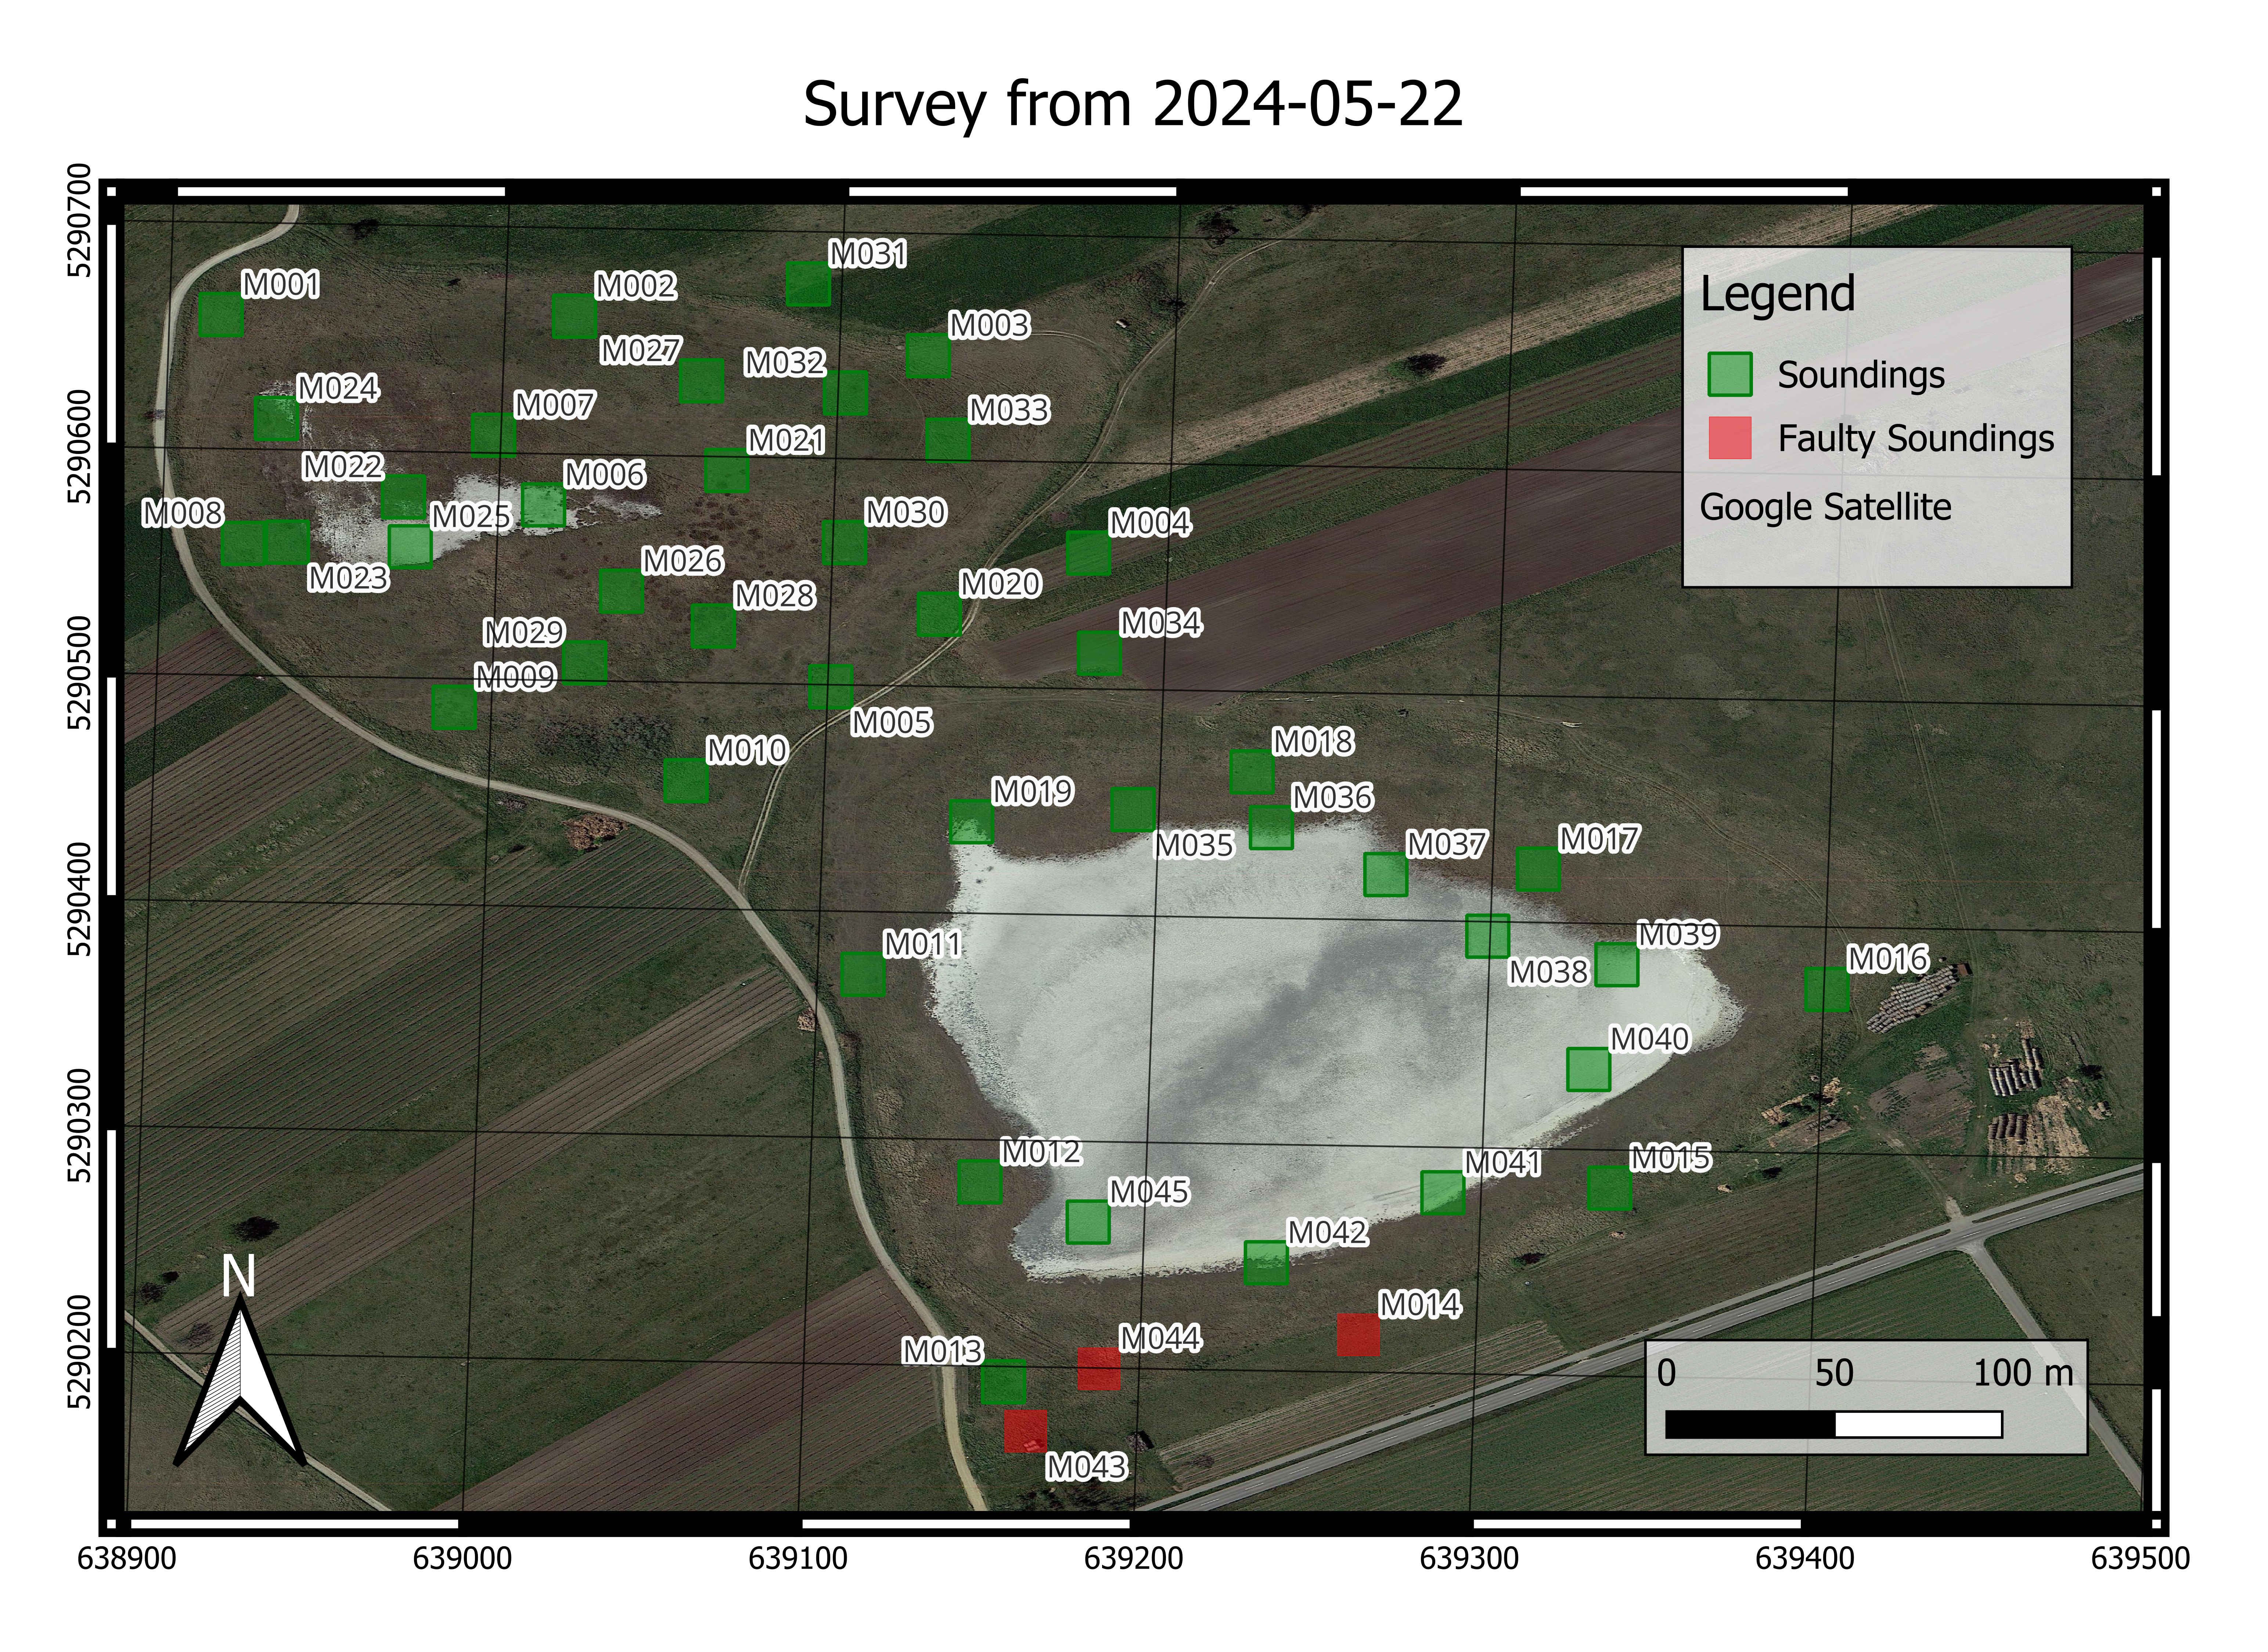
\includegraphics[width=\textwidth]{data/20240522/Survey_20240522}
    \caption{Numerically modelled typical TEM reponse with the signal a) and the apparent resistivity b).}
    \label{fig:survey_may}
\end{figure*}

\subsection{Experimental Set up}\label{subsec:set-up}
The L-Curve method was implemented for the inversion of TEM data and tested in a study site.

\subsubsection{Field Survey}\label{subsubsec:field-survey}
The field measurements were carried out at the Martenhofer Lacke in the Nationalpark Neusiedlersee - Seewinkel (16° 51' 23.058'' N, 47° 45' 8.4348'' E).
This site is located on the east side of the Neusiedler See, Austria.
The Martenhofer Lacke belongs to the soda lakes, which are characterised by a high salt content in the water.
Because this site is part of the national park, it can be assumed that it is a low noise environment.
For this work, two separate surveys were conducted: One on the 22nd May 2024 with 45 soundings and a second one on 8th October 2024 with 66 soundings.
Both surveys were done with the TEM-FAST 48 system manufactured by Applied Electromagnetic Research (AEMR) with a single-loop configuration.
In the survey in May, a $12.5\times12.5\,\text{m}$ loop was combined with a current of $1.0\,\text{A}$ for all soundings except for the first two (M001 and M002), where $4.1\,\text{A}$ were used.
For the first 14 soundings (M001-M014), 28 time windows were observed, resulting in a time range of $4-480\,\mu\text{s}$, and 4992 stacks.
For all other soundings (M015-M045), 24 time windows were observed, resulting in a time range of $4-240\,\mu\text{s}$, and 9984 stacks.
In the survey in October, a $6.25\times6.25\,\text{m}$ loop was used with a current of $4.1\,\text{A}$.
For all soundings, a time range of $4-240\,\mu\text{s}$(24\,\text{time windows}) were combined with 16640 stacks.


\subsubsection{Inversion Algorithm}\label{subsubsec:inversion}